\documentclass[12pt]{article}
\usepackage[a4paper,landscape,margin=1.5cm]{geometry} % Adjust margin as desired

% Packages for math symbols and functions
\usepackage{amsmath}
\usepackage{amssymb}
\usepackage{amsfonts}

% Package for rendering functions
\usepackage{mathrsfs}
\usepackage{pgfplots}
\usepackage{multicol}

% Adjust the font size for section headers
\usepackage{sectsty}
\sectionfont{\large\bfseries}

% Fancy Header
\usepackage{fancyhdr}
\pagestyle{fancy}
\fancyhf{} % Clear all header and footer fields
\lhead{\textsf{\textbf{HSLU Zulassungsstudium Formelsammlung}}}
\rhead{\textsf{Kevin Häusler}}
\title{\textsf{\textbf{HSLU Zulassungsstudium Formelsammlung}}}

% Tables
\usepackage{tabularx}

% Temp
\setlength{\columnseprule}{0.1pt} % Set the thickness of the line

% Define a command for displaying a function
\newcommand{\function}[2]{\ensuremath{\mathscr{#1}\left(#2\right)}}

% Define additional commands, if needed
% \newcommand{\commandname}{command definition}

\begin{document}


% Section Allgemein
\section*{Allgemein}
\begin{multicols}{3}
\subsection*{Wachstum und Verfall}
\textbf{Wachtsumsfaktor:}
\begin{equation*}
    q = 100\ \% + p\ \% = 1 + \frac{p}{100}
\end{equation*} 
\textbf{Verdoppelungszeit:}
\begin{equation*}
    t_V = \frac{\ln(2)}{\ln(q)}
\end{equation*}
\textbf{Abnahme:}
\begin{equation*}
    B(t) = {\color{red}m} \cdot t + b \quad \text{mit } {\color{red}m < 0}
\end{equation*}

\subsection*{Summe und Produkte}
\textbf{Summezeichen:} \\
Es sei:  n, k $\in$ Z und n $\geq$ k
\begin{equation*}
    \sum_{k=1}^{n} a_k = a_1 + a_2 + a_3 + \ldots + a_n 
\end{equation*}
\textbf{Produktzeichen:}
\begin{equation*}
    \prod_{k=1}^{n} a_k = a_1 \cdot a_2 \cdot a_3 \cdot \ldots \cdot a_n
\end{equation*}
k = Laufvariable, Laufindex  \\
1 = Startwert  n = Endwert\\
$a_{k}$ ist die Funktion bezueglich der Laufvariable \\

\subsection*{Aussagen, Logik, Mengen}
\begin{tabularx}{\columnwidth} {
        | >{\raggedright\arraybackslash}c
        | >{\raggedright\arraybackslash}X |}
    \hline
    \textbf{*}            & \textbf{Bedeutung}                                           \\ \hline
    $\varnothing$ oder {} & Leere Menge                        \\ \hline
    $x\in A$              & Element x ist in Menge A                          \\ \hline
    $x\notin A$           & Element x ist nicht in Menge A                    \\ \hline
    $A\subset B$          & A ist eine Teilmenge von B                                   \\ \hline
    $A\cap B$             & Schnittmenge von A und B                                     \\ \hline
    $A\cup B$             & Vereinigunsgsmenge von A und B                               \\ \hline
    $A\backslash B$       & Differenzbildung, Menge A ohne B                         \\\hline
    $\bar{A}_B$           & $:= \{x \,|\, x \in B \enspace \wedge \enspace x \notin A\}$ \\\hline
\end{tabularx}


\def\firstcircle{(0,0) circle (1cm)}
    \def\secondcircle{(0:1.2cm) circle (1cm)}

    \colorlet{circle edge}{blue!50}
    \colorlet{circle area}{blue!20}

    \tikzset{filled/.style={fill=circle area, draw=circle edge, thick},
        outline/.style={draw=circle edge, thick}}

    \setlength{\parskip}{5mm}
    % Set A and B
    \begin{tikzpicture}
        \begin{scope}
            \clip \firstcircle;
            \fill[filled] \secondcircle;
        \end{scope}
        \draw[outline] \firstcircle node {$A$};
        \draw[outline] \secondcircle node {$B$};
        \node[anchor=south] at (current bounding box.north) {$A \cap B$};
    \end{tikzpicture}
    \begin{tikzpicture}
        \draw[filled] \firstcircle node {$A$}
        \secondcircle node {$B$};
        \node[anchor=south] at (current bounding box.north) {$A \cup B$};
    \end{tikzpicture}

    % Set A but not B
    \begin{tikzpicture}
        \begin{scope}
            \clip \firstcircle;
            \draw[filled, even odd rule] \firstcircle node {$A$}
            \secondcircle;
        \end{scope}
        \draw[outline] \firstcircle
        \secondcircle node {$B$};
        \node[anchor=south] at (current bounding box.north) {$A\backslash  B$};
    \end{tikzpicture}
    \begin{tikzpicture}
        \draw[filled, even odd rule] \firstcircle node {$A$}
        \secondcircle node{$B$};
        \node[anchor=south] at (current bounding box.north) {$\overline{A \cap B}$};
    \end{tikzpicture}\\
    \textbf{Aussagenlogik:}\\
    Eine Aussage beschreibt einen Sachverhalt (durch Worte oder Symbole), der
    entweder wahr oder falsch ist.\\

    \scriptsize
    \begin{tabular}{@{ }c@{ }@{ }c | c@{ }@{ }c@{ }@{ }c@{ }@{ }c@{ }@{ }c | c@{ }@{ }c@{ }@{ }c@{ }@{ }c@{ }@{ }c | c@{ }@{ }c | c@{ }@{ }c@{ }@{ }c@{ }@{ }c@{ }@{ }c@{ }@{ }c}
        A & B &  & A & $\land$            & B &  &  & A & $\lor$             & B &  & $\lnot$            & B &  & A & $\lor$             & $\lnot$ & B & \\
        \hline
        T & T &  & T & \textcolor{red}{T} & T &  &  & T & \textcolor{red}{T} & T &  & \textcolor{red}{F} & T &  & T & \textcolor{red}{T} & F       & T & \\
        T & F &  & T & \textcolor{red}{F} & F &  &  & T & \textcolor{red}{T} & F &  & \textcolor{red}{T} & F &  & T & \textcolor{red}{T} & T       & F & \\
        F & T &  & F & \textcolor{red}{F} & T &  &  & F & \textcolor{red}{T} & T &  & \textcolor{red}{F} & T &  & F & \textcolor{red}{F} & F       & T & \\
        F & F &  & F & \textcolor{red}{F} & F &  &  & F & \textcolor{red}{F} & F &  & \textcolor{red}{T} & F &  & F & \textcolor{red}{T} & T       & F & \\
    \end{tabular}
    \normalsize

    \begin{tabularx}{\columnwidth} {
        | >{\raggedright\arraybackslash}c
        | >{\raggedright\arraybackslash}X
        | >{\raggedright\arraybackslash}c|}
    \hline
    \textbf{*}            & \textbf{Bedeutung}                        & \textbf{Beispiel}             \\ \hline
    $|A|$                 & Kardinalität/Mächtigkeit      & A = {1;2}                     \\
                          & Anzahl Elemente               & |$|A|$ = 2                    \\ \hline
    $\land$               & Konkuktion/UND A $\land$    & A $\land$ B                   \\ \hline
    $\lor$                & Disjunktion/ODER A $\lor$ B  = Wahr wenn  & {-1;0;1;}                     \\\hline
    $\neg$                & Negation A = W $\neg$A = F      & $\neg $A                      \\\hline
    $\implies$            & Implikation: Daraus folgt                 &                               \\ \hline
    $\Longleftrightarrow$ & äquivalenz  &                               \\ \hline
    $\forall$             & für Alle                                  & $\forall$ $x \in \mathbb{N}$  \\ \hline
    $\exists$             & Es Existiert                              & $\exists $ $x \in \mathbb{N}$ \\ \hline
    \end{tabularx}
\subsection*{Misc}

\newpage
\end{multicols}



% Section Gleichungen
\section*{Gleichungen}
\begin{multicols*}{3}
    \subsection*{Lineare Gleichung}
    \textbf{Definiton} \\
    Eine Gleichung, die sich in die Form $ax + b = 0$ bringen lässt, heisst lineare Gleichung. Wir können lineare Gleichungen daran erkennen, dass die Variable nur in der 1. Potenz auftritt, also kein $x^2$, $x^3$\dots enthalten. \\\\
    \textbf{Lösen einer Linearen Gleichung}
    \begin{enumerate}
        \item Gleichung nach $x$ auflösen
        \item Lösungsmenge aufschreiben
    \end{enumerate}
    \subsection*{Quadratische Gleichungen}
    \textbf{Definiton} \\
    Gleichungen, die sich auf die Form $ax^2 + bx + c = 0 \quad (a, b, c \in \mathbb{R}; a \neq 0)$
    bringen lassen, heissen quadratische Gleichungen. 
    \\~\\
    Wir können quadratische Gleichungen daran erkennen, dass die Variable $x$ in der 2. Potenz $x^2$, aber in keiner höheren Potenz vorkommt. 
    \\~\\
    Es gibt 4 Arten/Formen von Quadratischen Gleichungen.
    \begin{enumerate}
        \item $ax^2 + bx + c = 0 \quad (a, b, c \in \mathbb{R}; a \neq 0)$
        \item $ax^2 + bx = 0 \quad (a, b \in \mathbb{R}; a \neq 0)$
        \item $ax^2 + c = 0 \quad (a, c \in \mathbb{R}; a \neq 0)$
        \item $ax^2 = 0 \quad (a \in \mathbb{R}; a \neq 0)$
    \end{enumerate}
    \textbf{Lösung einer Reinquadratische Gleichung $ax^2 = 0$}\\~\\
    Reinquadratische Gleichungen ohne Absolutglied besitzen als einzige Lösung die Null.\\~\\
    \textbf{Lösung einer Reinquadratische Gleichung mit Absolutglied $ax^2 + c = 0$}

    \begin{enumerate}
        \item Gleichung nach $x^2$ auflösen
        \item Wurzel ziehen
        \item Lösungsmenge aufschreiben
    \end{enumerate}
    \textbf{Lösung einer Gemischtquadratische Gleichungen ohne Absolutglied $ax^2 + bx = 0$}

    \begin{enumerate}
        \item Quadratische Gleichung in Normalform bringen
        \item $x$ ausklammern
        \item  Faktoren gleich Null setzen
        \item Gleichung nach $x^2$ auflösen
        \item Lösungsmenge aufschreiben
    \end{enumerate}

    \subsection*{Mitternachtsformel}
    Gemischtquadratische Gleichungen $ax^2 + bx + c = 0$ mit Absolutglied lösen wir mit der Mitternachtsformel:
    \[x_{1/2} = \frac{-b \pm \sqrt{b^2 - 4ac}}{2a}\]
    \textbf{Fallunterscheidung:} \\
    \begin{align*}
        x_{1} &= \dfrac{-b - \sqrt{b^2 - 4ac}}{2a} \\
        x_{2} &= \dfrac{-b + \sqrt{b^2 - 4ac}}{2a}
    \end{align*}
    \textbf{Übersicht}\\~\\
    \begin{tabularx}{1.15\columnwidth} {
            | >{\raggedright\arraybackslash}X
            | >{\raggedright\arraybackslash}X
            | >{\raggedright\arraybackslash}X |}
        \hline
        \textbf{}                               & \textbf{Allgemeine Form}                       & \textbf{Normalform}                           \\ \hline
        Reinquadratisch ohne Absolutglied       & $2x^2 = 0$, $a = 2$, $b = 0$ und $c = 0$       & $x^2 = 0$, $a = 1$, $b = 0$ und $c = 0$       \\\hline
        Reinquadratisch mit Absolutglied        & $2x^2 -8 = 0$, $a = 2$, $b = 0$ und $c = -8$   & $x^2-4 = 0$, $a = 1$, $b = 0$ und $c = -4$    \\ \hline
        Gemischtquadrat- isch ohne Absolutglied & $2x^2-8x = 0$, $a = 2$, $b = -8$ und $c = 0$   & $x^2 -4x= 0$,  $a = 1$, $b = -4$ und $c = 0$  \\ \hline
        Gemischtquadrat- isch mit Absolutglied  & $2x^2-8x+6 = 0$, $a = 2$, $b = -8$ und $c = 6$ & $x^2-4x+3 = 0$, $a = 1$, $b = -4$ und $c = 3$ \\ \hline
    \end{tabularx}\\~\\
    \textbf{Regeln}\\~\\
    Wenn das lineare Glied fehlt, gilt b = 0. \\
    Wenn das absolute Glied fehlt, gilt c = 0. \\
    Wenn das $x^2$ allein steht, gilt a = 0 (wegen $1 \cdot x^2 = x^2$).\\
    Wenn das x allein steht, gilt b - 1(wegen $1 \cdot x = x$). \newpage
    \textbf{Lösen einer Quadratischen Gleichung mit Mitternachtsformel}
    \begin{enumerate}
        \item Gleichung in allgemeine Form bringen
        \item a,b,c aus der allgemeinen Form herauslesen
        \item a,b,c in die Mitternachtsformel einsetzen
        \item Lösung berechnen
        \item Lösungsmenge aufschreiben
    \end{enumerate}
    \subsection*{Bruchgleichungen}
    Wenn die Zähler der Brueche nur aus Zahlen bestehen, kann eine Kehrwertbildung sinnvoll sein.
    Den Kehrwert eines Bruchs erhält man durch Vertauschen von Zähler und Nenner.\\~\\
    \[\frac{{\colorbox{yellow}{$1$}}}{{\colorbox{orange}{$x$}}} = \frac{{\colorbox{yellow}{$2$}}}{{\colorbox{orange}{$x+1$}}} \Rightarrow  \frac{{\colorbox{orange}{$x$}}}{{\colorbox{yellow}{$1$}}} = \frac{{\colorbox{orange}{$x+1$}}}{{\colorbox{yellow}{$2$}}}\]
    \subsubsection*{Lösen einer Bruchgleichung}
    \begin{enumerate}
        \item Definitionsmenge bestimmen
        \item Gleichung nach $x$ auflösen
        \item Prïfen, ob der x-Wert in der Definitionsmenge ist
        \item Lösungsmenge aufschreiben
    \end{enumerate}
    \subsubsection*{Kehrwert}
    Wenn die Zähler der Brueche nur aus Zahlen bestehen, kann eine Kehrwertbildung sinnvoll sein.
    Den Kehrwert eines Bruchs erhält man durch Vertauschen von Zähler und Nenner.\\~\\
    \[\frac{{\colorbox{yellow}{$1$}}}{{\colorbox{orange}{$x$}}} = \frac{{\colorbox{yellow}{$2$}}}{{\colorbox{orange}{$x+1$}}} \Rightarrow  \frac{{\colorbox{orange}{$x$}}}{{\colorbox{yellow}{$1$}}} = \frac{{\colorbox{orange}{$x+1$}}}{{\colorbox{yellow}{$2$}}}\]


    \subsubsection*{Multiplikation übers Kreuz}
    Wenn auf beiden Seiten der Gleichung jeweils ein Bruch steht, kann eine Multiplikation ueber Kreuz sinnvoll sein.
    \[\frac{{\colorbox{yellow}{$1$}}}{{\colorbox{orange}{$x$}}} = \frac{{\colorbox{orange}{$2$}}}{{\colorbox{yellow}{$x+1$}}} \Rightarrow {\colorbox{yellow}{$1$}} \cdot {\colorbox{yellow}{$x+1$}} = {\colorbox{orange}{$2$}} \cdot {\colorbox{orange}{$x$}}\]

% AAAAAAAAAAAAAAA

\end{multicols*}



% Section Funtkionen
\section*{Funktionen}

\begin{multicols}{3}
    \subsection*{Lineare Funktion}
    \begin{center}
        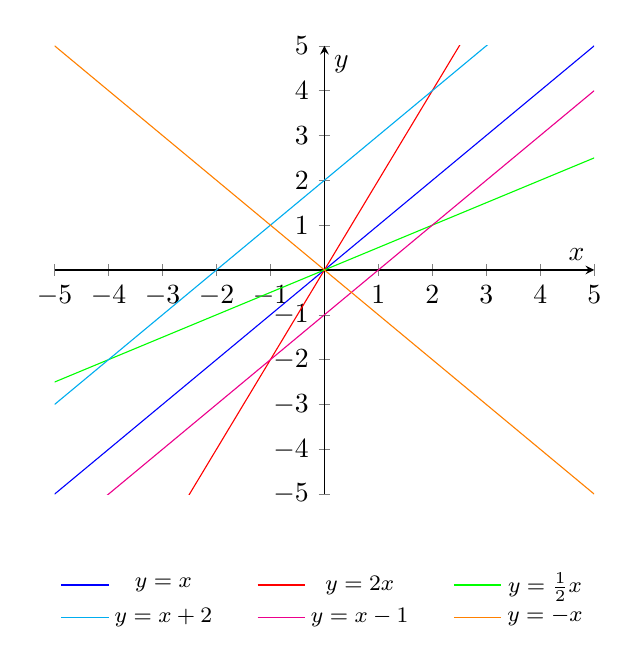
\begin{tikzpicture}
        \begin{axis}[
            axis lines=middle,
            xlabel=$x$,
            ylabel=$y$,
            xmin=-5,
            xmax=5,
            ymin=-5,
            ymax=5,
            xtick={-5,-4,-3,-2,-1,0,1,2,3,4,5},
            ytick={-5,-4,-3,-2,-1,0,1,2,3,4,5},
            legend pos=outer north east,
            legend style={
                draw=none,
                at={(0.5,-0.15)},
                anchor=north,
                legend columns=3,
                font=\footnotesize,
                /tikz/every even column/.append style={column sep=0.5cm},
            },
        ]
        
        % Linear Function: y = x
        \addplot[blue, domain=-5:5, samples=100] {x};
        \addlegendentry{$y = x$}
        
        % Transformed Functions
        \addplot[red, domain=-5:5, samples=100] {2*x};
        \addlegendentry{$y = 2x$}
        
        \addplot[green, domain=-5:5, samples=100] {0.5*x};
        \addlegendentry{$y = \frac{1}{2}x$}
        
        \addplot[cyan, domain=-5:5, samples=100] {x + 2};
        \addlegendentry{$y = x + 2$}
        
        \addplot[magenta, domain=-5:5, samples=100] {x - 1};
        \addlegendentry{$y = x - 1$}

        \addplot[orange, domain=-5:5, samples=100] {-x};
        \addlegendentry{$y = -x$}
        
        \end{axis}
        \end{tikzpicture}
    \end{center}
    \subsubsection*{Nullstelle berechnen}
    Funktion gleich Null setzen und nach X auflösen.
     \subsubsection*{Schnittpunkt berechnen}
    Beide Funktionen gleichsetzen, nach X auflösen und in eine der beiden Funktionen einsetzen um Y zu berechnen.

    \subsubsection*{Umkehrfunktion bilden}
    Funktion nach x auflösen, x und y vertauschen.
   
% Quadratic Function: y = x^2
\subsection*{Quadratische Funktion}
\begin{center}
    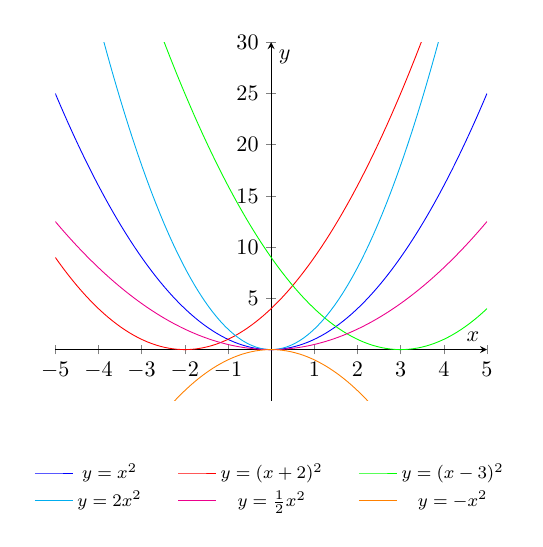
\begin{tikzpicture}[scale=0.8]
    \begin{axis}[
        axis lines=middle,
        xlabel=$x$,
        ylabel=$y$,
        xmin=-5,
        xmax=5,
        ymin=-5,
        ymax=30,
        xtick={-5,-4,-3,-2,-1,0,1,2,3,4,5},
        ytick={0,5,10,15,20,25,30},
        legend pos=outer north east,
            legend style={
                draw=none,
                at={(0.5,-0.15)},
                anchor=north,
                legend columns=3,
                font=\footnotesize,
                /tikz/every even column/.append style={column sep=0.5cm},
            },
    ]
    \addplot[blue, domain=-5:5, samples=100] {x^2};
    \addlegendentry{$y = x^2$}
    
    % Transformed Functions
    \addplot[red, domain=-5:5, samples=100] {(x+2)^2};
    \addlegendentry{$y = (x + 2)^2$}
    
    \addplot[green, domain=-5:5, samples=100] {(x-3)^2};
    \addlegendentry{$y = (x - 3)^2$}
    
    \addplot[cyan, domain=-5:5, samples=100] {2*x^2};
    \addlegendentry{$y = 2x^2$}
    
    \addplot[magenta, domain=-5:5, samples=100] {0.5*x^2};
    \addlegendentry{$y = \frac{1}{2}x^2$}

    \addplot[orange, domain=-5:5, samples=100] {-x^2};
    \addlegendentry{$y = -x^2$}
    
    \end{axis}
    \end{tikzpicture}
    \end{center}
    
    % Exponential Function: y = 2^x
    \subsection*{Exponential Funktion}
    \begin{center}
    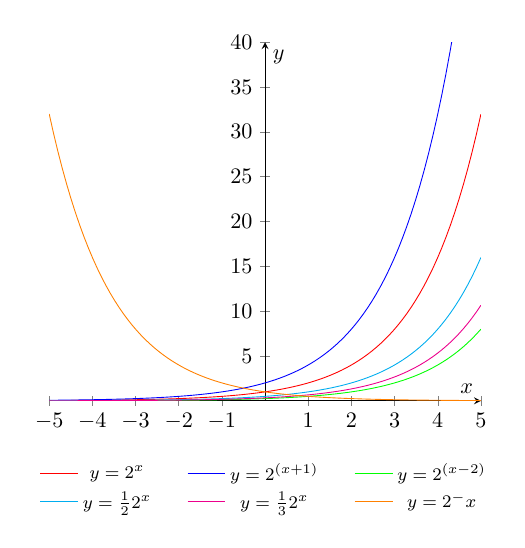
\begin{tikzpicture}[scale=0.8]
    \begin{axis}[
        axis lines=middle,
        xlabel=$x$,
        ylabel=$y$,
        xmin=-5,
        xmax=5,
        ymin=0,
        ymax=40,
        xtick={-5,-4,-3,-2,-1,0,1,2,3,4,5},
        ytick={0,5,10,15,20,25,30,35,40},
        legend pos=outer north east,
            legend style={
                draw=none,
                at={(0.5,-0.15)},
                anchor=north,
                legend columns=3,
                font=\footnotesize,
                /tikz/every even column/.append style={column sep=0.5cm},
            },
    ]
    \addplot[red, domain=-5:5, samples=100] {2^x};
    \addlegendentry{$y = 2^x$}
    
    % Transformed Functions
    \addplot[blue, domain=-5:5, samples=100] {2^(x+1)};
    \addlegendentry{$y = 2^{(x + 1)}$}
    
    \addplot[green, domain=-5:5, samples=100] {2^(x-2)};
    \addlegendentry{$y = 2^{(x - 2)}$}
    
    \addplot[cyan, domain=-5:5, samples=100] {0.5*2^x};
    \addlegendentry{$y = \frac{1}{2}2^x$}
    
    \addplot[magenta, domain=-5:5, samples=100] {2^x / 3};
    \addlegendentry{$y = \frac{1}{3}2^x$}

    \addplot[orange, domain=-5:5, samples=100] {2^-x};
    \addlegendentry{$y = 2^-x$}
    
    \end{axis}
    \end{tikzpicture}
    \end{center}
    
    \subsection*{Potenz Funktion}
    % Power Function: y = x^3
    \begin{center}
    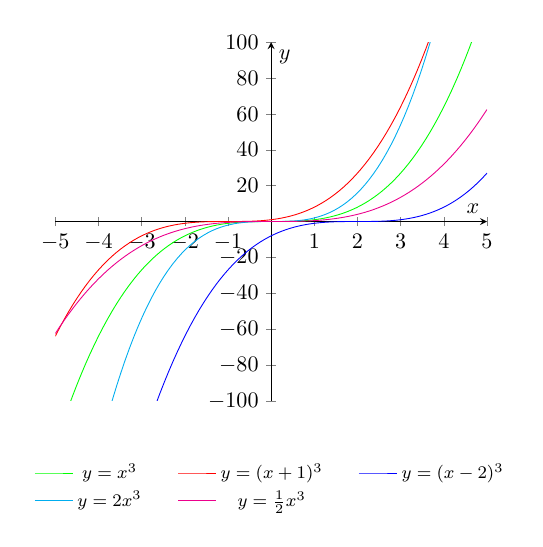
\begin{tikzpicture}[scale=0.8]
    \begin{axis}[
        axis lines=middle,
        xlabel=$x$,
        ylabel=$y$,
        xmin=-5,
        xmax=5,
        ymin=-100,
        ymax=100,
        xtick={-5,-4,-3,-2,-1,0,1,2,3,4,5},
        ytick={-100,-80,-60,-40,-20,0,20,40,60,80,100},
        legend pos=outer north east,
            legend style={
                draw=none,
                at={(0.5,-0.15)},
                anchor=north,
                legend columns=3,
                font=\footnotesize,
                /tikz/every even column/.append style={column sep=0.5cm},
            },
    ]
    \addplot[green, domain=-5:5, samples=100] {x^3};
    \addlegendentry{$y = x^3$}
    
    % Transformed Functions
    \addplot[red, domain=-5:5, samples=100] {(x+1)^3};
    \addlegendentry{$y = (x + 1)^3$}
    
    \addplot[blue, domain=-5:5, samples=100] {(x-2)^3};
    \addlegendentry{$y = (x - 2)^3$}
    
    \addplot[cyan, domain=-5:5, samples=100] {2*x^3};
    \addlegendentry{$y = 2x^3$}
    
    \addplot[magenta, domain=-5:5, samples=100] {0.5*x^3};
    \addlegendentry{$y = \frac{1}{2}x^3$}
    
    \end{axis}
    \end{tikzpicture}
    \end{center}
    
    \subsection*{Wurzel Funktion}
    % Square Root Function: y = sqrt(x)
    \begin{center}
    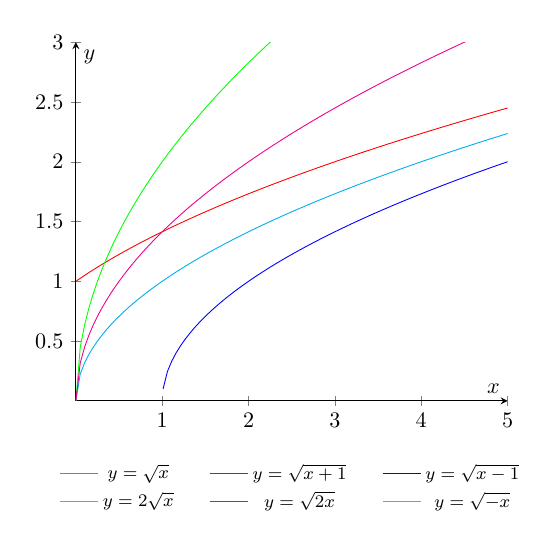
\begin{tikzpicture}[scale=0.8]
    \begin{axis}[
        axis lines=middle,
        xlabel=$x$,
        ylabel=$y$,
        xmin=0,
        xmax=5,
        ymin=0,
        ymax=3,
        xtick={0,1,2,3,4,5},
        ytick={0,0.5,1,1.5,2,2.5,3},
        legend pos=outer north east,
            legend style={
                draw=none,
                at={(0.5,-0.15)},
                anchor=north,
                legend columns=3,
                font=\footnotesize,
                /tikz/every even column/.append style={column sep=0.5cm},
            },
    ]
    \addplot[cyan, domain=0:5, samples=100] {sqrt(x)};
    \addlegendentry{$y = \sqrt{x}$}
    
    % Transformed Functions
    \addplot[red, domain=0:5, samples=100] {sqrt(x+1)};
    \addlegendentry{$y = \sqrt{x + 1}$}
    
    \addplot[blue, domain=0:5, samples=100] {sqrt(x-1)};
    \addlegendentry{$y = \sqrt{x - 1}$}
    
    \addplot[green, domain=0:5, samples=100] {2*sqrt(x)};
    \addlegendentry{$y = 2\sqrt{x}$}
    
    \addplot[magenta, domain=0:5, samples=100] {sqrt(2*x)};
    \addlegendentry{$y = \sqrt{2x}$}

    \addplot[orange, domain=0:5, samples=100] {sqrt(-x)};
    \addlegendentry{$y = \sqrt{-x}$}
    
    \end{axis}
    \end{tikzpicture}
    \end{center}
    
    \subsection*{Logarithmische Funktion}
    % Logarithmic Function: y = ln(x)
    \begin{center}
    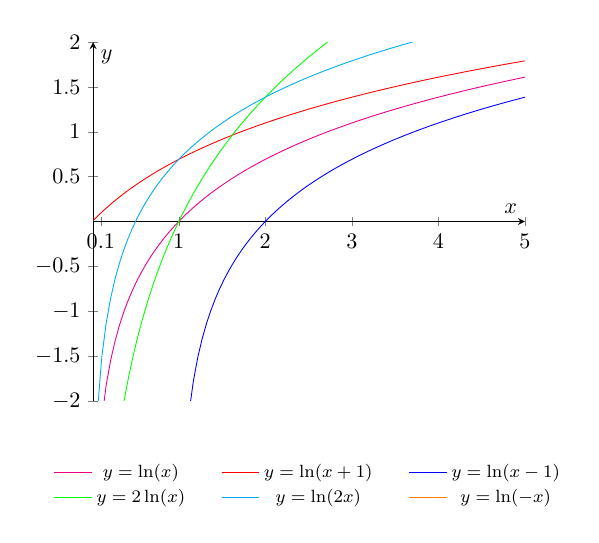
\begin{tikzpicture}[scale=0.8]
    \begin{axis}[
        axis lines=middle,
        xlabel=$x$,
        ylabel=$y$,
        xmin=0.01,
        xmax=5,
        ymin=-2,
        ymax=2,
        xtick={0.01,0.1,1,2,3,4,5},
        ytick={-2,-1.5,-1,-0.5,0,0.5,1,1.5,2},
        legend pos=outer north east,
            legend style={
                draw=none,
                at={(0.5,-0.15)},
                anchor=north,
                legend columns=3,
                font=\footnotesize,
                /tikz/every even column/.append style={column sep=0.5cm},
            },
    ]
    \addplot[magenta, domain=0.01:5, samples=100] {ln(x)};
    \addlegendentry{$y = \ln(x)$}
    
    % Transformed Functions
    \addplot[red, domain=0.01:5, samples=100] {ln(x+1)};
    \addlegendentry{$y = \ln(x + 1)$}
    
    \addplot[blue, domain=0.01:5, samples=100] {ln(x-1)};
    \addlegendentry{$y = \ln(x - 1)$}
    
    \addplot[green, domain=0.01:5, samples=100] {2*ln(x)};
    \addlegendentry{$y = 2\ln(x)$}
    
    \addplot[cyan, domain=0.01:5, samples=100] {ln(2*x)};
    \addlegendentry{$y = \ln(2x)$}

    \addplot[orange, samples=100] {ln(-x)};
    \addlegendentry{$y = \ln(-x)$}
    
    \end{axis}
    \end{tikzpicture}
    \end{center}
    \newpage
\end{multicols}

% Section Trigonometrie
\section*{Trigonometrie}
\begin{multicols}{3}

\small
\begin{multicols}{2}
\subsection*{Identitäten}

\textbf{Kofunktionen}
\begin{align*}
    & \sin(\frac{\pi}{2} - x) & = \cos x \\
    & \cos(\frac{\pi}{2} - x) & = \sin x \\
    & \tan(\frac{\pi}{2} - x) & = \cot x \\
    & \cot(\frac{\pi}{2} - x) & = \tan x \\
    & \sec(\frac{\pi}{2} - x) & = \csc x \\
    & \csc(\frac{\pi}{2} - x) & = \sec x
\end{align*}
\textbf{Symmetrie}
\begin{align*}
  \sin(-x) & = - \sin x \\
  \cos(-x) & = \cos x   \\
  \tan(-x) & = -\tan x
\end{align*}
\textbf{Doppelter Winkel}
\begin{align*}
  \sin(2x) & = 2 \sin x \cos x               \\
  \cos(2x) & = \cos^2 x - \sin^2 x           \\
           & = 2 \cos^2 x - 1                \\
           & = 1 - 2 \sin^2 x                \\
  \tan(2x) & = \frac{2 \tan x}{1 - \tan^2 x}
\end{align*}
\textbf{Halber Winkel}
\begin{align*}
  \sin \frac{x}{2} & = \pm \sqrt{ \frac{1 - \cos x }{2} } \\
  \cos \frac{x}{2} & = \pm \sqrt{ \frac{1 + \cos x }{2} } \\
  \tan \frac{x}{2} & = \frac{1 - \cos x }{\sin x}         \\
                   & = \frac{ \sin x }{ 1 + \cos x }
\end{align*}
\textbf{Exponent Reduktion}
\begin{align*}
  \sin^2 x & = \frac{1 - \cos 2x}{2}               \\
  \sin^4x  & = (\frac{1 - \cos 2x}{2})^2           \\
  \cos^2 x & = \frac{1 + \cos 2x}{2}               \\
  \cos^4x  & = (\frac{1 + \cos 2x}{2})^2           \\
  \tan^2 x & = \frac{1 - \cos 2x}{1 + \cos 2x}     \\
  \tan^4 x & =( \frac{1 - \cos 2x}{1 + \cos 2x})^2
\end{align*}
\textbf{Pythagoras}
\begin{align*}
  \sin^2 x + \cos^2 x & = 1        \\
  1 + \tan^2 x        & = \sec^2 x \\
  1 + \cot^2 x        & = \csc^2 x
\end{align*}
\textbf{Umkehrwert}
\begin{align*}
  \cot x & = \frac{1}{\tan x} \\
  \csc x & = \frac{1}{\sin x} \\
  \sec x & = \frac{1}{\cos x}
\end{align*}
\textbf{Quotient}
\begin{align*}
    \tan(x) = \frac{\sin(x)}{\cos(x)}\\
    \cot(x) = \frac{\cos(x)}{\sin(x)}
\end{align*}
\end{multicols}
\textbf{Summe und Differenz von Winkel}
\begin{align*}
  \sin(x + y) & = \sin x \cos y + \cos x \sin y             \\
  \sin(x - y) & = \sin x \cos y - \cos x \sin y             \\
  \cos(x + y) & = \cos x \cos y - \sin x \sin y             \\
  \cos(x - y) & = \cos x \cos y + \sin x \sin y             \\
  \tan(x + y) & = \frac{\tan x + \tan y}{1 - \tan x \tan y} \\
  \tan(x - y) & = \frac{\tan x - \tan y}{1 + \tan x \tan y}
\end{align*}
\textbf{Produkt zu Summe}
\begin{align*}
  \sin x \sin y & = \frac{1}{2}\big[\cos(x - y) - \cos(x + y)\big] \\
  \cos x \cos y & = \frac{1}{2}\big[\cos(x - y) + \cos(x + y)\big] \\
  \sin x \cos y & = \frac{1}{2}\big[\sin(x + y) + \sin(x - y)\big] \\
  \tan x \tan y & = \frac{ \tan x + \tan y }{ \cot x + \cot y }    \\
  \tan x \cot y & = \frac{ \tan x + \cot y }{ \cot x + \tan y }
\end{align*}
\textbf{Summe Zu Produkt}
\begin{align*}
  \sin x + \sin y & = 2 \sin \Big( \frac{x + y}{2} \Big) \cos \Big( \frac{x - y}{2} \Big)  \\
  \sin x - \sin y & = 2 \cos \Big( \frac{x + y}{2} \Big) \sin \Big( \frac{x - y}{2} \Big)  \\
  \cos x + \cos y & = 2 \cos \Big( \frac{x + y}{2} \Big) \cos \Big( \frac{x - y}{2} \Big)  \\
  \cos x - \cos y & = -2 \sin \Big( \frac{x + y}{2} \Big) \sin \Big( \frac{x - y}{2} \Big) \\
  \tan x + \tan y & = \frac{ \sin(x + y) }{ \cos x \cos y}                                 \\
  \tan x - \tan y & = \frac{ \sin(x - y) }{ \cos x \cos y}                                 \\
\end{align*}
\textbf{Additionstheoreme}
\begin{align*}
\includegraphics[scale=0.6]{trig/trig1.PNG}\\
\end{align*}
\textbf{Winkelfunktion des dreifachen winkel}
\begin{align*}
\includegraphics[scale=0.6]{trig/trig2.PNG}\\
\end{align*}
\newpage
\end{multicols}

% Section Vektoren
\section*{Vektoren}
\begin{multicols}{3}
\subsection*{Definition}
Ein Vektor ist durch Länge, Richtung und Orientierung eindeutig bestimmt.
\subsubsection*{Ortsvektor}
Ein Vektor, dessen Anfangspunkt im Ursprung O und dessen Endpunkt im Punkt A liegt, heißt Ortsvektor $\boldsymbol{\overrightarrow{OA}}$
von A.
\begin{equation*}
    A(x|y) \quad \Rightarrow \quad \overrightarrow{OA} = \begin{pmatrix} x \\ y \end{pmatrix}
\end{equation*}

\subsubsection*{Vektoraddition}
Vektoren lassen sich nur dann addieren, wenn sie gleicher Dimension und gleicher Art sind.
\begin{equation*}
    \vec{a}+\vec{b} = \begin{pmatrix} x_a \\ y_a\end{pmatrix}+\begin{pmatrix} x_b \\ y_b\end{pmatrix} = \begin{pmatrix} x_a+x_b \\ y_a+y_b\end{pmatrix}
\end{equation*}
\subsubsection*{Kommutativgesetz}
\begin{equation*}
    \vec{a}+\vec{b} = \vec{b}+\vec{a}
\end{equation*}
\subsubsection*{Assoziativgesetz}
\begin{equation*}
    (\vec{a}+\vec{b}) + \vec{c} = \vec{a} + (\vec{b}+\vec{c})
\end{equation*}

\subsubsection*{Vektorsubtraktion}
Vektoren werden subtrahiert, indem man ihre Komponenten subtrahiert:
\begin{equation*}
    \vec{a}-\vec{b} = \begin{pmatrix} x_a \\ y_a\end{pmatrix}-\begin{pmatrix} x_b \\ y_b\end{pmatrix} = \begin{pmatrix} x_a-x_b \\ y_a-y_b\end{pmatrix}
\end{equation*}

\subsection*{Skalar­multiplikation}
Wird ein Vektor $\vec{v}$ mit einem Skalar (einer reellen Zahl) $\lambda$ multipliziert, wird jede Komponente des Vektors mit dieser Zahl multipliziert:
\begin{equation*}
    \lambda \cdot \vec{v} = \lambda \cdot \begin{pmatrix} x \\ y \end{pmatrix} = \begin{pmatrix} \lambda \cdot x \\ \lambda \cdot y \end{pmatrix}
\end{equation*}
\subsubsection*{Misc}
Multipliziert man einen Vektor mit einem Skalar c, wird der Vektor – in Abhängigkeit des Wertes des Skalars – verlängert, verkürzt und/oder er ändert seine Orientierung.\\
$c > 1$: Der Vektor wird verlängert.\\
$0 < c < 1$: Der Vektor wird verkürzt.\\
$c < 0$: Der Vektor ändert seine Orientierung.\\

\subsection*{Betrag eines Vektors}
Die Länge eines Vektors heisst Betrag des Vektors.
\begin{equation*}
    \vec{v}= \begin{pmatrix} x \\ y \end{pmatrix} \Rightarrow \left|\vec{v}\right| = \sqrt{x^2 + y^2}
\end{equation*}

\subsection*{Einheitsvektor}
Ein Vektor der Länge 1 heisst Einheitsvektor.
\begin{equation*}
    \vec{a}^0 = \frac{1}{|a|} \vec{a}
\end{equation*}
\subsubsection*{Abstand zweier Punkte}
Verbindungsvektor berechnen und dann Länge des Vektors berechnen.
\subsection*{Skalarprodukt}
Das Skalarprodukt ist eine mathematische Verknüpfung, die zwei Vektoren eine Zahl (Skalar) zuordnet.
\begin{equation*}
    \vec{a} \circ \vec{b} = \begin{pmatrix} a_1 \\ a_2 \\ a_3 \end{pmatrix} \circ \begin{pmatrix} b_1 \\ b_2 \\ b_3 \end{pmatrix} = a_1 \cdot b_1 + a_2 \cdot b_2 + a_3 \cdot b_3
\end{equation*}
\subsubsection*{Kommutativgesetz}
\begin{equation*}
    \vec{a} \circ \vec{b} = \vec{b} \circ \vec{a}
\end{equation*}
\subsubsection*{Distributivgesetz}
\begin{equation*}
    \vec{a} \circ \left(\vec{b} + \vec{c}\right) = \vec{a} \circ \vec{b} + \vec{a} \circ \vec{c}
\end{equation*}
\subsubsection*{Gemischtes
Assoziativgesetz}
\begin{equation*}
    \left(k \cdot \vec{a}\right) \circ \vec{b} = k \cdot \left(\vec{a} \circ \vec{b}\right)
\end{equation*}
\subsection*{Winkel zwischen zwei Vektoren}

\begin{equation*}
    \cos\varphi = \frac{\vec{u}\circ\vec{v}}{\left|\vec{u}\right|\cdot\left|\vec{v}\right|} \qquad \Rightarrow \qquad \varphi = \cos^{-1}\left(\frac{\vec{u}\circ\vec{v}}{\left|\vec{u}\right|\cdot\left|\vec{v}\right|}\right)
\end{equation*}
Skalarprodukt berechnen, Beträge der Vektoren berechnen, Zwischenergebnisse in die Formel einsetzen und Formel nach Winkel auflösen.

\newpage

\end{multicols}

% Add more sections and formulas as needed

\end{document}
